%!TEX root = Thesis.tex

\chapter{Experimental}
\label{ch:expt}

\section{General procedures}
\label{section:generalprocedures}

\fixme{copied from Almas, check that the necessary info is here, everything is correct and everything unneccessary is removed}

All reactions and manipulation of products and reagents were carried out under an inert nitrogen atmosphere using standard Schlenk line techniques unless otherwise stated.  Analytical grade reagents and high purity solvents were degassed and purged with nitrogen before use, except for diethyl ether and tetrahydrofuran which were dried by refluxing over sodium/benzophenone ketyl.  

NMR spectra were recorded using a Varian Unity Inova 300 (300~MHz for \proton, 75~MHz for \carbon, 121~MHz for \phosphorus{} and 282~MHz for \fluorine), a Varian Unity Inova 500 (500~MHz for \proton{} and 125~MHz for \carbon), or a Varian DirectDrive 600 (600~MHz for \proton and 150~MHz for \carbon{}) spectrometers.   The 600~MHz instrument was equipped with a Varian inverse-detected triple-resonance HCN cold probe operating at 25~K.  All direct-detected \proton{} and \carbon{} chemical shifts were referenced to the residual solvent peak.\cite{Fulmer2010}  NMR samples were prepared under an inert nitrogen or argon atmosphere unless otherwise stated, using \ce{C6D6}, \ce{CDCl3}, \ce{CD2Cl2}, acetone-\ce{d6} and toluene-\ce{d8}.  All NMR solvents were degassed before use and stored under inert atmosphere over molecular sieves.  Variable temperature NMR was carried out in toluene-\ce{d8} or \ce{CD2Cl2} using Varian Unity Inova 300~MHz NMR spectrometer.  Infrared spectra were recorded with a PerkinElmer Spectrum One FT-IR spectrophotometer using pressed KBr discs.  Microanalyses were performed by The Campbell Microanalytical Laboratory at Otago University.  Melting points were recorded on a Gallenkamp Melting Point Apparatus under vacuum unless otherwise stated. Single crystal \textit{X}-ray diffraction data were recorded by the \textit{X}-ray Crystallography Laboratory at the University of Canterbury.  Electrospray ionisation mass spectra were either recorded on a PE Biosystem Mariner 5158 TOF mass spectrometer at Victoria University, or performed by the GlycoSyn QC laboratory at Industrial Research Limited using a Waters Q-TOF Premier Tandem mass spectrometer.  Calculated \proton{} NMR spectra were obtained from gNMR spectral simulation programme, version 5.0.6.0 written by P. H. M. Budzelaar, IvorySoft 2006.

\fixme{All reactions with silver were performed in tinfoil wrapped vessels to prevent degradation due to light}
\fixme{In the case of a 1:1 CDCl3:CD2Cl2 solvent mixing being used for NMR the spectra were referenced to the CD2Cl2 residual solvent peak}
%\subsection*{Crystallography} 
%\label{subsec:X-ray}

%Diffraction data\footnote{Bruker {\scriptsize{SMART}} (Version 5.054), {\scriptsize{SADABS}} (Version 2.03), and {\scriptsize{SAINT}} (Version 6.02A), Bruker AXS Inc., Madison, Wisconsin, USA, 1997.} (see Tables \ref{tab:dataPN582}, \ref{tab:dataPdPNCl2}, \ref{tab:datanbagostic}, \ref{tab:datadimer} for details) were collected using Bruker CCD diffractometers with Mo K$\alpha$ radiation (0.71073~\AA) from fine-focus sealed tubes with graphite monochromators, using phi and omega scans.  Multi-scan absorption corrections were applied.  The structures were solved by direct methods and full-matrix least squares refinement,\footnote{G. M. Sheldrick, {\scriptsize{SHELX-97}}.  Programmes for the Solution and Refinement of Crystal Structures, 1997.} with anisotropic thermal parameters for all non-H atoms.\cite{Sheldrick}  Hydrogen atoms are in calculated positions and refined using a riding model with {\scriptsize{SHELXL}} defaults.  The agostic hydrogen atom in \ce{Pt-H-C} interaction was located and its position refined, and all relevant bond distances and angles were calculated using Mercury, version 1.4.2.  Molecular drawings were made using ORTEP3.\cite{ORTEP}

\section{Ligands and Non-Transition Metal Derivatives}
\label{section:experimental:ligands}

%\pagevalues

%%%%%
%S-tBu %
%%%%%
%\newpage{}
\subsection*{2,8-Dimethyl-4,6-bis(di-\emph{tert}-butylphosphino)phenoxathiin \\(\emph{t}-Bu-thixantphos)}

\begin{structure}
\begin{center}
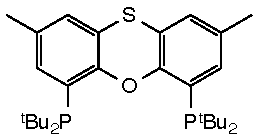
\includegraphics{../Structures/StBuligand.pdf}
\end{center}
\end{structure}

\noindent{}\emph{sec}-Butyllithium (29.8 mL, 1.0 M in cyclohexane, 29.8 mmol) was added dropwise to a stirred solution of 2,8-dimethylphenoxathiin (2.27 g, 9.94 mmol) and TMEDA (4.47 mL, 29.8 mmol) in diethyl ether (96 mL) at -78\degC{}.  The resulting yellow solution was warmed to at room temperature and stirred for a further 16 hours over which time a dark red colour developed.  The reaction was cooled to -78\degC{} and chlorodi-\emph{t}-butylphosphine (5.67 mL, 29.8 mmol) was added dropwise.  The reaction mixture was stirred for a further seven days resulting in a yellow solution with a white precipitate of lithium chloride.  The solvent was removed \emph{in vacuo} giving an orange oil.  This oil was taken up in dichloromethane (25 mL) and washed with water (3 x 15 mL).  The organic layer was passed through a column of magnesium sulfate and solvent was removed \emph{in vacuo}.  The product was purified by dissolving in hot \emph{n}-propanol and cooling at \fixme{temperature} giving small white crystals (1.33 g, 26\%).  This compound can be handled in the air for short periods however, should be stored under an inert atmosphere.
\Phosphorusintro{CDCl3}
\NMRPsinglet{9.5}.
\Protonintro{500}{\fixme{CDCl3}}
\NMRsinglet{7.29}{\StBucH},
\NMRsinglet{6.88}{\StBuaH},
\NMRsinglet{2.25}{\StBugH},
\NMRmultiplet{1.22-1.24}{\StBuiH}.
\Carbonintro{125}{\fixme{CDCl3}}
\NMRPC{155.3}{vt}{13.0}{\StBueC},
\NMRsinglet{134.6}{\StBucC},
\NMRsinglet{131.9}{\StBubC},
\fixme{something at 128?},
\NMRsinglet{127.4}{\StBuaC},
\NMRPC{120.1}{vt}{2.4}{\StBufC},
\fixme{tBu groups},
\NMRPC{30.8}{vt}{9.1}{\StBuiC},
\NMRsinglet{20.9}{\StBugC}.
HRMS calcd for \ce{C30H47OP2S} [M+H]$^+$ \emph{m/z} = 517.2817; found = 517.2819.
\fixme{IR, EA}

%%%%%
%Si-tBu%
%%%%%
%\newpage{}
\subsection*{4,6-bis(di-\emph{tert}-butylphosphino)-10,10-dimethylphenoxasilin \\(\emph{t}-Bu-sixantphos)}

\begin{structure}[h]
\begin{center}
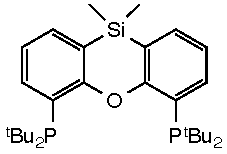
\includegraphics{../Structures/SitBuligand.pdf}
\end{center}
\end{structure}

This compound was prepared similarly to \fixme{reference to S-tBu ligand} using 10,10-dimethylphenoxasilin (0.40 g, 1.8 mmol) giving white crystals (0.127 g, 14\%).
\Phosphorusintro{CD2Cl2}
8.42 (s, \XJXX{4}{PSi} = 4.8 Hz).
%\NMRPsinglet{8.42} \fixme{it has silicon satellites? should I add them?}.
\Protonintro{500}{CD2Cl2}
\NMRcoupled{7.87}{d}{7.4}{\SitBucH},
\NMRcoupled{7.53}{d}{7.1}{\SitBuaH},
\NMRcoupled{7.12}{t}{7.5}{\SitBubH},
\NMRPH{1.29}{vt}{5.6}{\SitBuiH},
\NMRsinglet{0.46}{\SitBugH},
\Carbonintro{125}{CD2Cl2}
\NMRPC{164.3}{vt}{11.3}{\SitBueC},
\NMRsinglet{138.5}{\SitBucC},
\NMRsinglet{134.8}{\SitBuaC},
\NMRsinglet{\fixme{128}}{\SitBudC},
\NMRsinglet{121.4}{\SitBubC},
\NMRsinglet{119.4}{\SitBufC},
\NMRPC{33.2}{\fixme{dd}}{16.3, 13.9}{\SitBuhC},
\NMRPC{31.0}{vt}{9.6}{\SitBuiC},
\NMRsinglet{-0.09}{\SitBugC}.
HRMS calcd for \ce{C30H49OP2Si} [M + H]$^+$ \emph{m/z} = 515.3022; found = 515.3021.
\fixme{IR, EA}

\fixme{change the NMR data so it goes from large to small}

%%%%%
%C-tBu%
%%%%%

\subsection*{9,9-Dimethyl-4,6-bis(diphenylphosphino)xanthene \\(\tBuxantphos)}

\begin{structure}[h]
\begin{center}
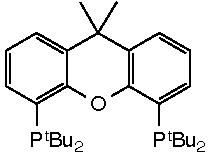
\includegraphics{../Structures/CtBuligand.pdf}
\end{center}
\end{structure}

Dissolved 9,9-dimethylxanthene (0.50 g, 2.38 mmol) and \gls{TMEDA} (1.07 mL, 7.13 mmol) in diethyl ether (20 mL).  Added s-BuLi drop wise causing the reaction to change to yellow then a deep red.  After stirring for 24 hours chlorodi-(\emph{tert}-butyl)phosphine (1.36 mL, 7.13 mmol) was added dropwise.  After six days of stirring a white precipitate had formed and a pale yellow solution remained.  The solvent was removed \emph{in vacuo} and the resulting yellow oil was taken up in dichloromethane (20 mL) and washed with degassed water (10 mL).  The aqueous layer was further extracted with dichloromethane (20 mL) and the combined organic layers were washed with water (3 x 10 mL).  The organic layers were dried over magnesium sulfate and the solvent was removed \emph{in vacuo}.  The resulting pale yellow solid was recrystallised from n-propanol yielding the title compound as fine white needles (0.44 g, 37\%).

The \proton{} and \carbon{} NMR data are consistent with the literature values.\cite{Mispelaere2005}  However, the literature reported \phosphorus{} chemical shift is 12.4 ppm.  Due to this discrepancy full characterisation data for this compound is given below.

\Phosphorusintro{CDCl3}
\NMRPsinglet{10.2},
\Protonintro{500}{CDCl3}
\NMRcoupled{7.60}{d}{7.6}{\CtBucH},
\NMRdd{7.38}{7.8}{1.5}{\CtBuaH},
\NMRcoupled{7.03}{t}{7.6}{\CtBubH},
\NMRsinglet{1.57}{\CtBuhH},
\NMRmultiplet{1.21-1.25}{\CtBujH}.
\Carbonintro{125}{CDCl3}
\NMRPC{155.8}{vt}{12.0}{\CtBueC},
\NMRbsinglet{133.7}{\CtBucC},
\NMRPC{130.7}{vt}{2.0}{\CtBufC},
\NMRPC{126.6}{dd}{21.6, 15.4}{\CtBudC},
\NMRsinglet{125.5}{\CtBuaC},
\NMRsinglet{121.5}{\CtBubC},
\NMRbsinglet{35.0}{\CtBugC},
\NMRPC{32.7}{dd}{16.1, 12.7}{\CtBuiC},
\NMRsinglet{31.1}{\CtBuhC},
\NMRPC{30.8}{vt}{9.4}{\CtBujC}.
HRMS calcd for \ce{C31H49OP2} [M+H]$^+$ \emph{m/z} = 499.3253; found = 499.3241.

%%%%%%%%
% C-tBu acid %
%%%%%%%%
\subsection*{Protonated 4,6-bis(di-\emph{tert}-butylphosphino)-9,9-dimethylxanthene\\(\emph{t}-Bu-xantphos) with \ce{CH2(SO2CF3)2}}

\begin{structure}[h]
\begin{center}
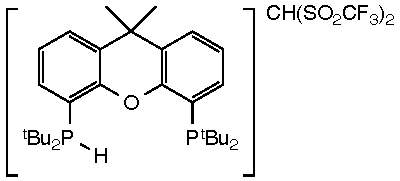
\includegraphics{../Structures/CtBuH.pdf}
\end{center}
\end{structure}

%Reaction3013

%Phosphorus
\Phosphorusintro{CDCl3}
\NMRbsinglet{17.4}
%Proton

\Protonintro{600}{CDCl3}
\NMRPH{8.57}{vt}{470.6}{P\emph{H}}, \fixme{kind of not really}
\NMRmultiplet{7.67-7.74}{4H, Ar},
\NMRbsinglet{7.39}{2H, Ar},
\NMRbsinglet{4.06}{C\emph{H}\ce{(SO2CF3)2}}, \fixme{check this is there},
\NMRsinglet{1.65}{\CtBuhH},
\NMRmultiplet{1.37-1.43}{\CtBujH}.
%Fluorine
\Fluorineintro{CDCl3}
\NMRsinglet{-80.9}{C\emph{F}\sub{3}}
%Carbon
\Carbonintro{150}{CDCl3}
\NMRmultiplet{153.6-153.8}{\CtBueC},
\NMRbcarbon{132.5},
\NMRbcarbon{130.3},
\NMRbcarbon{125.0},
\NMRCF{121.0}{quartet}{317.9}{CH\ce{(SO2}\emph{C}\ce{F3)2}},
\NMRsinglet{54.1}{\emph{C}H\ce{(SO2CF3)2}},
\NMRsinglet{35.5}{\CtBugC},
\NMRbsinglet{34.0}{\CtBuiC},
\NMRsinglet{30.8}{\CtBuhC},
\NMRbsinglet{29.4}{\CtBujC}.
HRMS calcd for \ce{C31H49OP2} [M]$^+$ \emph{m/z} = 499.3253; found = 499.3254.



%%%%%%%
%S-tBu acid%
%%%%%%%
\subsection*{Protonated 2,8-Dimethyl-4,6-bis(di-\emph{tert}-butylphosphino)phenoxathiin \\(\emph{t}-Bu-thixantphos) with \ce{CH2(SO2CF3)2}}

\begin{structure}[h]
\begin{center}
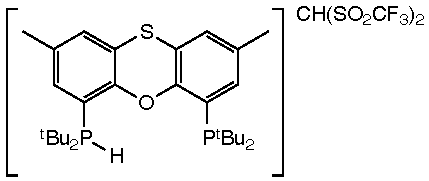
\includegraphics{../Structures/StBuH.pdf}
\end{center}
\end{structure}

%Reaction 1093
2,8-Dimethyl-4,6-bis(di-\emph{tert}-butylphosphino)phenoxathiin \\(\emph{t}-Bu-thixantphos) and \ce{CH2(SO2CF3)2} were combined in an NMR tube and dissolved in \ce{CD2Cl2}.  

\Phosphorusintro{CD2Cl2}
\NMRPsinglet{15.8}
\Protonintro{500}{CD2Cl2}
\NMRmultiplet{8.99}{P\emph{H}},
\NMRsinglet{7.29}{\StBuaH},
\NMRsinglet{7.22}{\StBucH},
\NMRsinglet{3.83}{\ce{C\emph{H}(SO2CF3)}},
\NMRsinglet{2.36}{\StBugH},
\NMRmultiplet{1.41-1.44}{\StBuiH}.
\Carbonintro{125}{\fixme{CD2Cl2}}
\NMRsinglet{152.9}{\StBueC},
\NMRsinglet{136.2}{\StBubC},
\NMRsinglet{132.5}{\StBuaC},
\NMRsinglet{131.8}{\StBucC},
\NMRsinglet{122.2}{\StBufC},
\NMRCF{121.5}{quartet}{325.6}{\ce{CF3}},
\NMRsinglet{115.3}{\StBudC},
\NMRsinglet{34.4}{\StBuhC},
\NMRsinglet{29.5}{\StBuiC}.
One peak (\emph{C}\ce{H(SO2CF3)}) obscured by solvent.
HRMS calcd for \ce{C30H47OP2S} [M]$^+$ \emph{m/z} = 517.2817; found = 517.2817.

\fixme{IR, EA, MS}

%%%%%%%%
% Si-tBu acid %
%%%%%%%%
\subsection*{Protonated 4,6-bis(di-\emph{tert}-butylphosphino)-10,10-dimethylphenoxasilin\\(\emph{t}-Bu-Sixantphos) with \ce{CH2(SO2CF3)2}}

\begin{structure}[h]
\begin{center}
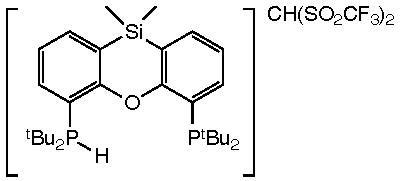
\includegraphics{../Structures/SitBuH.pdf}
\end{center}
\end{structure}

%Reaction4010\\
4,6-bis(di-\emph{tert}-butylphosphino)-10,10-dimethylphenoxasilin (\emph{t}-Bu-Sixantphos) and \ce{CH2(SO2CF3)2} were combined in an NMR tube and dissolved in \ce{CDCl3}.  

%Phosphorus
\Phosphorusintro{CDCl3}
\NMRPsinglet{14.3}
%Proton
\Protonintro{500}{CDCl3}
\NMRmultiplet{9.57}{P\emph{H}},
\NMRmultiplet{7.85-7.87}{\SitBucH},
\NMRHH{7.79}{d}{6.6}{\SitBuaH},
\NMRHH{7.41}{t}{7.5}{\SitBubH},
\NMRbsinglet{4.06}{C\emph{H}\ce{(SO2CF3)2}},
\NMRPH{1.43}{vt}{7.5}{\SitBuiH},
\NMRsinglet{0.53}{\SitBugH}.
%Fluorine
\Fluorineintro{CDCl3}
\NMRsinglet{-80.8}{C\emph{F}\sub{3}}
%Carbon
\Carbonintro{125}{CDCl3}
\NMRPC{161.5}{vt}{5.3}{\SitBueC},
\NMRsinglet{139.1}{\SitBuaC},
\NMRsinglet{136.9}{\SitBucC},
\NMRPC{124.0}{vt}{2.4}{\SitBubC},
\NMRsinglet{121.1}{\SitBufC},
\NMRCF{121.1}{quartet}{327.2}{CH\ce{(SO2}\emph{C}\ce{F3)2}},
\NMRbsinglet{115.0}{\SitBudC},
\NMRsinglet{53.6}{\emph{C}H\ce{(SO2CF3)2}},
\NMRPC{34.2}{vt}{3.9}{\SitBuhC},
\NMRPC{29.5}{vt}{4.3}{\SitBuiC},
\NMRsinglet{-0.4}{\SitBugC}.
HRMS calcd for \ce{C30H49OP2Si} [M]$^+$ \emph{m/z} = 515.3022; found = 515.3023.


\fixme{IR, EA, MS}

%%%%%%
%CtBu Se%
%%%%%%

%Reaction4031, 6010
\subsection*{9,9-Dimethyl-4,6-bis(di\emph{tert}-butylphosphino)xanthene selenide}
\fixme{Correct this name}
\begin{structure}[h]
\begin{center}
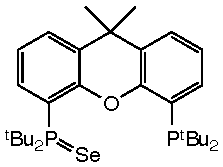
\includegraphics{../Structures/CtBuSe.pdf}
\end{center}
\end{structure}

A solution of \tBuxantphos{} (0.041 g, 0.082 mmol) in toluene (5 mL) was added to grey selenium (0.130 g, 1.65 mmol) in toluene (5 mL).  The reaction was heated to reflux with stirring for 3 days.  The resulting yellow solution was allowed to cool, filtered and reduced \emph{in vacuo} to give a pale yellow solid (0.038 g, 80\%).    

\Phosphorusintro{1:1, CDCl3:CD2Cl2}
\NMRPsinglet{10.2},
\NMRPasysinglet{10.6}{P},
\NMRPasysinglet{101.9}{P=Se}.
\Protonintro{500}{1:1 CDCl3:CD2Cl2}
\NMRdd{9.26}{17.4}{7.8}{P(=Se)CC\emph{H}},
\NMRcoupled{7.67}{d}{7.6}{\CtBucH},
\NMRcoupled{7.60}{d}{7.5}{P(=Se)CCCC\emph{H}},
\NMRcoupled{7.50}{d}{7.5}{PCCCC\emph{H}},
\NMRcoupled{7.24}{t}{7.8}{P(=Se)CCC\emph{H}},
\NMRcoupled{7.19}{t}{7.6}{\CtBubH},
\NMRcoupled{1.66}{d}{16.6}{\ce{P(=Se)C(C\emph{H3})3}},
\NMRsinglet{1.57}{\CtBuhH},
\NMRcoupled{1.19}{d}{11.8}{\CtBujH}.
\Carbonintro{125}{1:1, CDCl3:CD2Cl2},
\NMRPC{157.0}{d}{21.1}{\CtBueC},
\NMRsinglet{154.2}{P(=Se)C\emph{C}O},
\NMRPC{143.5}{d}{11.6}{P(=Se)C\emph{C}H},
\NMRsinglet{136.0}{\CtBucC},
\NMRsinglet{132.8}{PCC\emph{C}C(bridge)},
\NMRPC{132.0}{d}{4.8}{P(=Se)CC\emph{C}C(bridge)},
\NMRPC{129.2}{d}{2.4}{P(=Se)CCC\emph{C}H},
\NMRsinglet{126.3}{PCCC\emph{C}H},
\NMRPC{125.3}{d}{35}{\CtBudC},
\NMRsinglet{123.2}{2C, P(=Se)CC\emph{C}H, PCC\emph{C}H},
\NMRPC{115.4}{d}{39.8}{P(=Se)\emph{C}(Ar)},
\NMRPC{39.2}{d}{34.6}{P(=Se)\emph{C}(CH3)3},
\NMRsinglet{35.3}{\emph{C}(bridge)},
\NMRPC{33.5}{d}{26.9}{\CtBuiC},
\NMRPC{31.2}{d}{15.4}{\CtBujC}.
\NMRdd{30.9}{7.7}{2.0}{P(=Se)C(\emph{C}\ce{H3)3}},
\NMRsinglet{30.8}{C(bridge)\emph{C}\ce{H3}}.
HRMS calcd for \ce{C31H49OP2Se} [M+H]$^+$ \emph{m/z} = 579.2421; found = 579.2381.

\section{Silver Complexes}
\label{section:experimental:silver}

%%%%%%
%StBu Se%
%%%%%%

%Reaction4026, 6009
\subsection*{2,8-Dimethyl-4,6-bis(di-\emph{tert}-butylphosphino)phenoxathiin \\(\emph{t}-Bu-thixantphos) selenide}
\fixme{Correct this name}
\begin{structure}[h]
\begin{center}
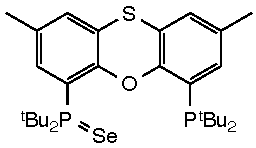
\includegraphics{../Structures/StBuSe.pdf}
\end{center}
\end{structure}

A solution of \tButhixantphos{} (0.042 g, 0.081 mmol) in toluene (5 mL) was added to grey selenium (0.128 g, 1.62 mmol) in toluene (5 mL).  The reaction was heated to reflux with stirring for 3 days.  The resulting yellow solution was allowed to cool, filtered and reduced \emph{in vacuo} to give the title compound as a yellow solid (0.047 g, 98\%).   
HRMS calcd for \ce{C31H49OP2SSe} [M+H]$^+$ \emph{m/z} = 597.1984; found = 597.1919.

%%%%%%
%SitBu Se%
%%%%%%

%Reaction6008
\subsection*{4,6-bis(di-\emph{tert}-butylphosphino)-10,10-dimethylphenoxasilin \\(\emph{t}-Bu-sixantphos) selenide}
\fixme{Correct this name}
\begin{structure}[h]
\begin{center}
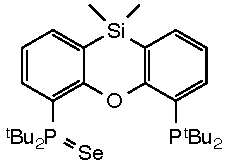
\includegraphics{../Structures/SitBuSe.pdf}
\end{center}
\end{structure}

A solution of \tBuXantphos{} (0.031 g, 0.060 mmol) in toluene (5 mL) was added to grey selenium (0.095 g, 1.20 mmol) in toluene (5 mL).  The reaction was heated to reflux with stirring for 3 days.  The resulting yellow solution was allowed to cool, filtered and reduced \emph{in vacuo} to give a pale yellow solid (0.036 g, 100\%).
HRMS calcd for \ce{C30H49OP2SeSi} [M+H]$^+$ \emph{m/z} = 595.2190; found = 595.2172.


%%%%%%
%AgCl StBu%
%%%%%%

%Reaction3002
%\newpage{}

\subsection*{\emph{t}-Bu-thixantphossilverchloride, 3003} \fixme{check name}

\begin{structure}[h]
\begin{center}
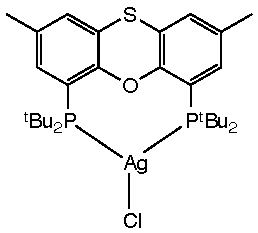
\includegraphics{../Structures/StBuSilverChloride.pdf}
\end{center}
\end{structure}

This reaction was carried out in the dark.  \fixme{StBu ligand} (88 mg, 0.17 mmol) and silver chloride (24 mg, 0.17 mmol) were combined \ce{CH2Cl2} (4 mL) in a Schlenk tube.  After 5 days stirring the solution was passed through a plug of alumina, washing with dichloromethane (4 x 1 mL).  The solvent was removed in vacuo giving a cloudy oil.  The oil was triturated with hexane (2 mL) yielding the title compound as a white powder (94 mg, 84\%).  The resulting silver complex is light sensitive and care should be taken to exclude light.

\fixme{check if in vacuo should be italicised} 

%Phosphorus
\Phosphorusintro{CDCl3}
\NMRAgP{21.81}{406.7}{469.6}.
%Proton
\Protonintro{600}{CDCl3}
\NMRPH{7.39}{d}{1.0}{\StBucH},
\NMRPH{7.11}{d}{1.6}{\StBuaH},
\NMRsinglet{2.31}{\StBugH}
\NMRmultiplet{1.41}{\StBuiH}.
%Carbon
\Carbonintro{150}{CDCl3}
\NMRPC{155.5}{vt}{6.6}{\StBueC},
\NMRPC{134.8}{d}{4.9}{\StBucC},
\NMRPC{133.1}{d}{1.5}{\StBubC},
\NMRsinglet{130.3}{\StBuaC},
\NMRPC{122.8}{vt}{3.0}{\StBufC},
\NMRmultiplet{120.9}{\StBudC}, \fixme{virtual quartet?}
\NMRmultiplet{35.3}{\StBuhC}, \fixme{virtual quartet?}
\NMRPC{30.9}{vt}{5.6}{\StBuiC},
\NMRsinglet{20.8}{\StBugC}.
HRMS calcd for \ce{C30H46OP2SAg} [M-Cl]$^+$ \emph{m/z} = 623.1796; found = 623.1805.

\fixme{IR, EA, MS}
\fixme{Check frequency of 13C on 600 MHz}

%%%%%%%%
% AgCl SitBu %
%%%%%%%%

%Reaction3003
%\newpage{}
\subsection*{\emph{t}-Bu-Sixantphossilverchloride} \fixme{check name}
\begin{structure}[h]
\begin{center}
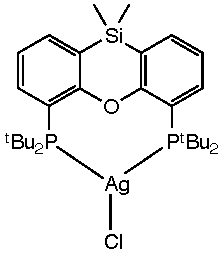
\includegraphics{../Structures/SitBuSilverChloride.pdf}
\end{center}
\end{structure}

This reaction was carried out in the dark.  Combined \fixme{SitBu ligand} and silver chloride in an NMR tube and dissolved in \ce{CDCl3} and sonicated for 5 mins.  After four days the reaction was sonicated for 6 x 5 mins.  Decanted the solution and washed the solid with dichloromethane (3 x 1 mL).  The solution was removed \emph{in vacuo} yielding the title compound as a white solid (31 mg, 97\%).  The resulting silver complex is light sensitive and care should be taken to exclude light.

%Phosphorus
\Phosphorusintro{CDCl3}
\NMRAgP{24.2}{408.1}{471.1}
%Proton
\Protonintro{600}{CDCl3}
\NMRmultiplet{7.88}{\SitBucH},
\NMRdd{7.61}{7.0}{1.8}{\SitBuaH},
\NMRHH{7.21}{t}{7.3}{\SitBubH},
\NMRmultiplet{1.42}{\SitBuiH},
\NMRsinglet{0.46}{\SitBugH}.
%Carbon
\Carbonintro{150}{CDCl3}
\NMRPC{163.9}{vt}{5.2}{\SitBueC},
\NMRPC{138.2}{d}{4.4}{\SitBucC},
\NMRsinglet{136.3}{\SitBuaC},
\NMRsinglet{122.2}{\SitBufC},
\NMRsinglet{122.1}{\SitBubC},
\NMRmultiplet{120.5}{\StBudC}, \fixme{quartet?}
\NMRmultiplet{35.5}{\StBuhC}, \fixme{quartet?}
\NMRPC{31.0}{vt}{5.6}{\StBuiC},
\NMRsinglet{-1.3}{\StBugC}.
HRMS calcd for \ce{C30H48OP2Ag} [M-Cl]$^+$ \emph{m/z} = 621.2001; found = 621.2021.

\fixme{IR, mass spec, EA}


%%%%%%%
%AgCl CtBu%
%%%%%%%

%Reaction3017
%\newpage{}
\subsection*{\emph{t}-Bu-xantphossilverchloride} \fixme{check name}

\begin{structure}[h]
\begin{center}
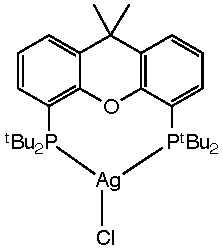
\includegraphics{../Structures/CtBuSilverChloride.pdf}
\end{center}
\end{structure}

This reaction was carried out in the dark as silver chloride and the product are light sensitive.  Combined \fixme{CtBu ligand} (17 mg, 0.034 mmol) and silver chloride (5 mg, 0.035 mmol) in an NMR tube and dissolved in \ce{CDCl3}.  After 48 hours sonicated 10 x 5 mins, decanted the solution from the solid and vacced to dryness leaving a white powder.  \fixme{yield}

%Phosphorus
\Phosphorusintro{CDCl3}
\NMRAgP{20.7}{409.3}{472.2}
%Proton
\Protonintro{500}{CDCl3}
\NMRPH{7.68}{d}{6.9}{\CtBucH},
\NMRdd{7.53}{7.6}{1.2}{\CtBuaH},
\NMRHH{7.19}{t}{7.7}{\CtBubH},
\NMRsinglet{1.56}{\CtBuhH},
\NMRmultiplet{1.40-1.43}{\CtBujH}.
%Carbon
\Carbonintro{125}{CDCl3}
\NMRPC{156.5}{vt}{6.5}{\CtBueC},
\NMRmultiplet{133.7}{\CtBucC},
\NMRPC{130.7}{vt}{\CtBufC},
\NMRsinglet{126.8}{\CtBuaC},
\NMRPC{122.7}{d}{\fixme{?}}{\CtBubC},
\NMRsinglet{119.3}{\CtBudC},
\NMRPC{35.6}{\fixme{?}}{vt}{\CtBugC},
\NMRPC{35.1}{\fixme{?}}{vt}{\CtBuiC},
\NMRPC{30.8}{vt}{5.6}{\CtBujC},
\NMRsinglet{28.5}{\CtBuhC}.
HRMS calcd for \ce{C31H48OP2Ag} [M-Cl]$^+$ \emph{m/z} = 605.2226; found = 605.2163.


\fixme{Need to check and get all of the couplings}
\fixme{Make sure that all of the proton couplings around all of the rings have consistent PH or HH}
\fixme{Consider using numbering}

%%%%%%%%%
% AgBF4 SitBu %
%%%%%%%%%

%Reaction3009
\subsection*{(\tBuSixantphos)silver tetrafluoroborate}
\begin{structure}[h]
\begin{center}
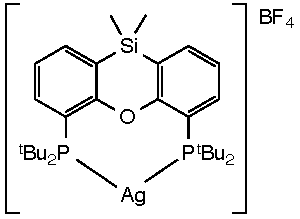
\includegraphics{../Structures/SitBuSilverBF4.pdf}
\end{center}
\end{structure}
Combined \tBusixantphos{} (0.027 g, 0.052 mmol) and silver tetrafluoroborate (0.010, 0.052 mmol) in an NMR tube and dissolved in \ce{CDCl3}.  After 3 days the reaction was complete by NMR.  Decanted the solution into a Schlenk flask and removed the solvent in vacuo yielding the title compound as a white solid (0.024 g, 0.034 mmol, 64\%)

%Phosphorus
\Phosphorusintro{CDCl3}
\NMRAgP{31.5}{482.9}{557.4}
%Proton
\Protonintro{500}{CDCl3}
\NMRbsinglet{7.84}{\SitBucH},
\NMRHH{7.73}{d}{6.8}{\SitBuaH},
\NMRHH{7.34}{t}{7.3}{\SitBubH},
\NMRPH{1.40}{vt}{15.9}{\SitBuiH},
\NMRsinglet{0.49}{\SitBugH}.
%Carbon
\Carbonintro{125}{CDCl3}
\NMRPC{162.3}{vt}{8.7}{\SitBueC},
\NMRsinglet{138.2}{\SitBuaC},
\NMRPC{138.1}{d}{6.7}{\SitBucC},
\NMRPC{123.1}{d}{1.9}{\SitBubC},
\NMRsinglet{122.1}{\SitBufC},
\NMRmultiplet{118.4}{\SitBudC},
\NMRmultiplet{35.7}{\SitBuhC}, %Virtual triplet of doublet?
\NMRmultiplet{30.9}{\SitBuiC},
\NMRsinglet{-0.6}{\SitBugC}.
%Fluorine
\Fluorineintro{CDCl3}
\NMRsinglet{-152.2}{\ce{BF4-}}.
HRMS calcd for \ce{C30H48OP2AgSi} [M-\ce{BF4-}]$^+$ \emph{m/z} = 621.2001; found = 621.2032.

%%%%%%%%
%AgBF4 StBu%
%%%%%%%%

%Reaction3008
%\newpage{}

\subsection*{(\tBuThixantphos)silver tetrafluoroborate}

\begin{structure}[h]
\begin{center}
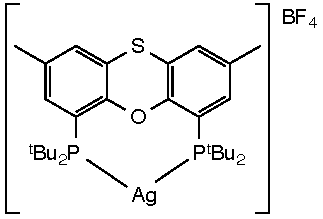
\includegraphics{../Structures/StBuSilverBF4.pdf}
\end{center}
\end{structure}

A solution of \tButhixantphos{} (0.026 g, 0.050 mmol) in 0.5 mL of deutero-chloroform was added to silver tetrafluoroborate (0.010 g, 0.051 mmol) in an NMR tube.  After 3 days the reaction NMR showed complete conversion into the title complex.  Decanted the solution into a Schlenk flask and removed the solvent in vacuo yielding the product as a white solid (0.030 g, 0.042 mmol, 84\%).

%Phosphorus
\Phosphorusintro{CDCl3}
\NMRAgP{28.4}{486.7}{562.2}.
%Proton
\Protonintro{500}{CDCl3}
\NMRsinglet{7.32}{\StBucH},
\NMRsinglet{7.16}{\StBuaH},
\NMRsinglet{2.33}{\StBugH},
\NMRPH{1.40}{vt}{15.8}{\StBuiH}.
%Carbon
\Carbonintro{125}{CDCl3}
\NMRPC{153.9}{vt}{11.0}{\StBueC},
\NMRPC{134.4}{d}{\fixme{??}}{\StBubC},
\NMRPC{134.2}{d}{6.30}{\StBucC},
\NMRsinglet{131.1}{\StBuaC},
\NMRsinglet{122.3}{\StBufC},
\NMRmultiplet{119.4}{\StBudC}, %virtual triplet of doublets?
\NMRmultiplet{35.5}{\StBuhC},
\NMRmultiplet{30.8}{\StBuiC},
\NMRsinglet{20.7}{\StBugC}.
HRMS calcd for \ce{C30H46OP2SAg} [M-\ce{BF4-}]$^+$ \emph{m/z} = 623.1796; found = 623.1826.

\fixme{IR, EA}

%%%%%%%%
%AgBF4 CtBu%
%%%%%%%%

%Reaction3016
%\newpage{}
\subsection*{(\tBuXantphos)silver tetrafluoroborate} %\fixme{check name}

\begin{structure}[h]
\begin{center}
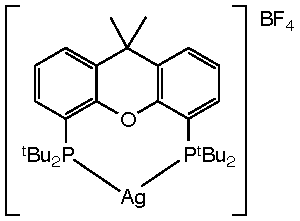
\includegraphics{../Structures/CtBuSilverBF4.pdf}
\end{center}
\end{structure}
This reaction was carried out in the dark as silver compounds are typically light sensitive.  Combined \tBuxantphos{} (0.017 g, 0.034 mmol) and silver tetrafluoroborate (0.008 g, 0.041 mmol) in an NMR tube and dissolved in \ce{CDCl3}.  After 48 hours the reaction was complete by NMR.  Decanted the solution into another flask and removed the solvent in vacuo yielding a white solid in quantitative yield.  

%Phosphorus
\Phosphorusintro{CDCl3}
\NMRAgP{27.6}{486.3}{561.1}
%Proton
\Protonintro{500}{CDCl3}
\NMRmultiplet{7.63-7.67}{\CtBuaH, \CtBucH},
\NMRHH{7.29}{t}{7.7}{\CtBubH},
\NMRsinglet{1.59}{\CtBuhH},
\NMRmultiplet{1.39-1.42}{\CtBujH}.
%Carbon
\Carbonintro{125}{CDCl3}
\NMRPC{154.9}{vt}{5.6}{\CtBueC},
\NMRPC{133.5}{vt}{1.9}{\CtBucC},
\NMRPC{133.5}{d}{5.8}{\CtBufC},
\NMRsinglet{128.4}{\CtBuaC},
\NMRsinglet{123.8}{\CtBubC},
\NMRsinglet{117.8}{\CtBudC},
\NMRPC{35.6}{vtd}{5.3, 2.4}{\CtBugC},
\NMRPC{35.3}{\fixme{d,d,d?}}{4.8, 2.7, 7.6}{\CtBuiC},
\NMRPC{30.6}{\fixme{d,d,d?}}{5.3, 4.4, 6.5 }{\CtBujC},
\NMRsinglet{29.4}{\CtBuhC}.
%Fluorine
\Fluorineintro{CDCl3}
\NMRsinglet{-152.0ppm}{\ce{BF4-}}
HRMS calcd for \ce{C31H48OP2Ag} [M-Cl]$^+$ \emph{m/z} = 605.2226; found = 605.2217.


%\fixme{Need to check and get all of the couplings}
%\fixme{Make sure that all of the proton couplings around all of the rings have consistent PH or HH}
%\fixme{Consider using numbering}
%\fixme{check how on earth to write up all of the tBu couplings...}

%%%%%%%%
%PdCl2 StBu %
%%%%%%%%
%\newpage{}
%\subsection*{\emph{t}-Bu-thixantphospalladiumdichloride, 2020} \fixme{check name}
%\begin{structure}[h]
%\begin{center}
%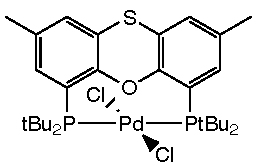
\includegraphics{../Structures/PdCl2(s(tBu)2)_complex.pdf}
%\end{center}
%\end{structure}

%\fixme{StBu ligand} (36 mg, 0.070 mmol) and \ce{[Pd(COD)Cl2]} (20 mg, 0.070 mmol) were combined in an NMR tube and dissolved in \ce{C6D6} and heated to 60\degC{} for 48 hours.  The solvent was removed in vacuo yielding the title compound as a dark red solid (37 mg, 77\%).

%Phosphorus
%\Phosphorusintro{C6D6}
%\NMRPsinglet{41.9}
%Proton
%\Protonintro{500}{C6D6}
%\NMRsinglet{7.17}{PC(Ar)\emph{H}},
%\NMRsinglet{7.15}{SCC\emph{H}}
%\NMRsinglet{2.33}{C(Ar)\ce{C\emph{H}3}}
%\NMRPH{1.59}{vt}{7.1}{PCC\emph{H}\sub{3}}
%Carbon
%\Carbonintro{125}{CDCl3}
%\NMRPC{155.1}{vt}{4.8}{\emph{C}O}
%\NMRsinglet{134.4}{PC(Ar)\emph{C}H}
%\NMRPC{133.4}{vt}{\fixme{?}}{\emph{C}(Ar)\ce{CH3}}
%\NMRsinglet{130.4}{SC\emph{C}H})
%\NMRmultiplet{123.5}{P\emph{C}(Ar)}
%\NMRPC{123.1}{vt}{3.0}{\emph{C}S}
%\NMRPC{39.5}{vt}{5.8}{P\emph{C}C\ce{H3}}
%\NMRsinglet{31.2}{PC\emph{C}\ce{H3}}
%\NMRsinglet{20.7}{C(Ar)\emph{C}\ce{H3}}

%\fixme{IR, EA, 1H, 31P, 13C, MS}
%\fixme{Redraw complex with new parameters}
%\fixme{Check solvent}

\section{Platinum Complexes}
\label{section:experimental:platinum}

%%%%%%
% PtStBu %
%%%%%%

\subsection*{\emph{t}-Bu-Thixantphosplatinum}
\begin{structure}[h]
\begin{center}
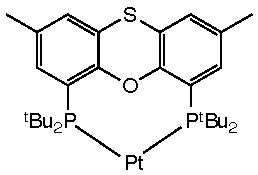
\includegraphics{../Structures/StBuPlatinum.pdf}
\end{center}
\end{structure}

\subsubsection{Starting from Pt(COD)2}
\subsubsection{Starting from Pt(nb)3}

\Phosphorusintro{C6D6}
\NMRPPt{78.6}{4809.5}
\Protonintro{600}{C6D6}
\NMRPH{7.32}{d}{1.8}{\StBucH},
\NMRsinglet{6.87}{\StBuaH},
\NMRsinglet{1.95}{\StBugH},
\NMRPH{1.52}{vt}{13.8}{\StBuiH}.
\Carbonintro{150}{C6D6}
\NMRPC{155.9}{vt}{10.4}{\StBueC},
\NMRsinglet{133.3}{\StBucC},
\NMRPC{132.1}{vt}{5.2}{\StBubC},
\NMRsinglet{128.8}{\StBuaC},
\NMRPC{126.6}{vt}{28.9}{\StBudC},
\NMRPC{126.1}{vt}{5.8}{\StBufC},
\NMRPC{37.8}{vt}{15}{\StBuhC},
\NMRPC{31.7}{vt}{10.4}{\StBuiC},
\NMRsinglet{20.5}{\StBugC}.
\fixme{IR, EA, MS}


%%%%%%%%
% PtStBu(nb) %
%%%%%%%%

\subsection*{\emph{t}-Bu-Thixantphosplatinumnorbornene}
\begin{structure}[h]
\begin{center}
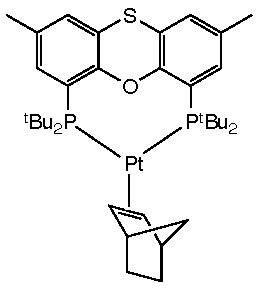
\includegraphics{../Structures/StBuPlatinumnorbornene.pdf}
\end{center}
\end{structure}

\Phosphorusintro{C6D6}
\NMRPPt{55.6}{3612}
\Protonintro{600}{C6D6}
\NMRsinglet{7.61}{\StBucH},
\NMRsinglet{6.95}{\StBuaH},
\NMRsinglet{3.12}{nb CH},
\NMRPtH{2.37}{bs}{1}{67.8}{nb =C\emph{H}},
\NMRsinglet{1.96}{\StBugH},
\NMRobscuredH{1.93}{COSY}{2H}{nb C\emph{H}\sub{2}},
\NMRmultiplet{1.42-1.56}{\StBuiH},
\NMRobscuredH{1.32}{COSY}{3H}{nb C\emph{H}\sub{2}, bridge \ce{CH2}},
\NMRHH{0.62}{d}{15.3}{1H, nb bridge \ce{CH2}}.
\Carbonintro{150}{C6D6}
\NMRPC{158.9}{vt}{9.8}{\StBueC},
\NMRPtC{135.4}{s}{2}{26.6}{\StBucC},
\NMRbsinglet{130.9}{\StBubC},
\NMRbsinglet{130.7}{\StBuaC},
\NMRPC{127.6}{vt}{5.8}{\StBufC},
\NMRbsinglet{125.9}{\StBudC},
\NMRPtC{51.9}{bs}{1}{343.9}{nb =\emph{C}H},
\NMRsinglet{44.9}{nb \emph{C}H},
\NMRmultiplet{38.5}{\StBuhC},
\NMRobscuredC{38.0-38.5}{HSQC}{nb bridge \emph{C}\ce{H2}},
\NMRbsinglet{31.7}{\StBuiC},
\NMRPtC{31.4}{bs}{3}{61.4}{nb \emph{C}\ce{H2}},
\NMRsinglet{20.7}{\StBugC}.
\fixme{IR, EA, MS}

%%%%%%%%%
% PtStBuC2H4 %
%%%%%%%%%
\subsection*{\emph{t}-Bu-Thixantphosplatinumethene}
\begin{structure}[h]
\begin{center}
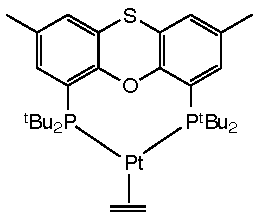
\includegraphics{../Structures/StBuPlatinumethene.pdf}
\end{center}
\end{structure}

\Phosphorusintro{C6D6}
\NMRPPt{55.7}{3899}
\Protonintro{600}{C6D6}
\NMRsinglet{7.63}{\StBucH},
\NMRsinglet{6.96}{\StBuaH},
\NMRPtH{2.50}{bs}{1}{59.5}{\ce{C=C\emph{H\sub{2}}}},
\NMRsinglet{1.97}{\StBugH},
\NMRmultiplet{1.38-1.40}{\StBuiH}.
\Carbonintro{150}{C6D6}
\NMRbsinglet{158.7}{\StBueC},
\NMRPtC{135.3}{s}{2}{29.5}{\StBucC},
\NMRbsinglet{131.0}{\StBubC},
\NMRbsinglet{130.5}{\StBuaC},
\NMRPC{128.5}{vt}{5.8}{\StBufC},
\NMRbsinglet{125.7}{\StBudC},
\NMRmultiplet{38.7}{\StBuhC},
\NMRPtC{34.2}{bs}{1}{223.2}{\ce{C=C}}
\NMRbsinglet{31.6}{\StBuiC},
\NMRsinglet{20.7}{\StBugC}.
\fixme{IR, EA, MS}

%%%%%%%
%PtStBuO2%
%%%%%%%
\subsection*{\emph{t}-Bu-Thixantphosplatinumdioxygen}
\begin{structure}[h]
\begin{center}
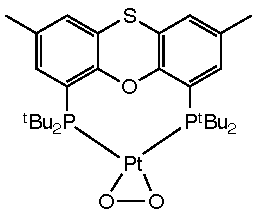
\includegraphics{../Structures/StBuPtO2.pdf}
\end{center}
\end{structure}

\Phosphorusintro{CD2Cl2}
\NMRPPt{38.4}{4488}
\Protonintro{600}{CD2Cl2}
\NMRcoupled{7.59}{dd}{5.9, 1.0}{a},
\NMRsinglet{7.32}{c},
\NMRsinglet{2.34}{g},
\NMRPH{1.43}{d}{14.4}{C(Ar)\ce{C\emph{H}3}},
\Carbonintro{125}{CD2Cl2}
\NMRbsinglet{156.6}{\emph{C}O},
\NMRPtC{133.8}{s}{2}{37.9}{PC(Ar)\emph{C}H},
\NMRPC{133.1}{d}{5.3}{\emph{C}(Ar)\ce{CH3}},
\NMRbsinglet{131.7}{SCC\emph{C}(\ce{CH3})},
\NMRsinglet{128.5}{\emph{C}S},
\NMRPC{119.3}{d}{27.8}{P\emph{C}(Ar)},
\NMRPC{39.3}{d}{23.5}{P\emph{C}\ce{CH3}},
\NMRPC{31.2}{d}{5.3}{PC\emph{C}\ce{H3}},
\NMRsinglet{21.2}{C(Ar)\emph{C}\ce{H3}}.
\fixme{IR, EA, MS}

\subsubsection{Starting from Pt(C2H4)}
\subsubsection{Starting from 14-electron}

%%%%%%%%
% Metallated  %
%%%%%%%%
\subsection*{Metallated complex}
\begin{structure}[h]
\begin{center}
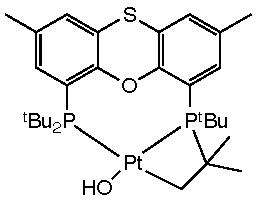
\includegraphics{../Structures/Metallated.pdf}
\end{center}
\end{structure}

\Phosphorusintro{CD2Cl2}
\NMRPtwoPt{38.17}{s}{1794}{\ce{P}-\textsuperscript{t}\ce{Bu2}}
\NMRPtwoPt{$-$49.63}{s}{3943}{\ce{PCCPt}}
\Protonintro{600}{CD2Cl2}
\NMRPH{7.60}{d}{3.8}{c2}
\NMRsinglet{7.25}{a1}
\NMRsinglet{7.16}{a2}
\NMRPH{6.95}{d}{6.5}{c1}
\NMRsinglet{2.34}{g1}
\NMRsinglet{2.32}{g2}
\NMRPH{1.71}{d}{12.9}{i3}
\NMRcoupled{1.41}{d}{15.9}{k}
\NMRcoupled{1.36}{d}{14.9}{l}
\NMRPH{1.34}{d}{13.2}{i2}
\NMRmultiplet{1.2-1.5, obscured}{m}
\NMRPH{1.03}{d}{15.0}{i1}
\Carbonintro{150}{CD2Cl2}
\NMRPC{157.1}{d}{9.0}{e2}
\NMRPC{153.9}{d}{4.3}{e1}
\NMRPC{134.2}{d}{3.2}{c2}
\NMRPC{133.8}{d}{6.3}{b1}
\NMRPC{133.4}{d}{3.2}{b2}
\NMRsinglet{132.8}{c1}
\NMRPC{130.5}{d}{1.6}{a1}
\NMRPC{129.6}{d}{1.6}{a2}
\NMRPC{128.5}{dd}{4.2, 1.6}{f1}
\NMRPC{124.0}{d}{4.3}{f2}
\NMRPC{121.3}{d}{13.8}{d2}
\NMRPC{116.6}{dd}{30.7, 1.6}{d1}
\NMRPC{46.7}{d}{37.6}
\NMRPC{40.8}{d}{10.1}{h2}
\NMRPC{36.8}{d}{8.0}{h3}
\NMRPC{36.0}{d}{22.3}{h1}
\NMRPC{33.2}{d}{5.8}{i3}
\NMRsinglet{32.6}{l}
\NMRPC{32.1}{dd}{10.1, 3.7}{k}
\NMRPC{31.3}{d}{5.3}{i2}
\NMRbsinglet{28.8}{i1}
\NMRsinglet{21.3}{g2}
\NMRsinglet{21.0}{g1}
\fixme{\NMRsinglet{15.7}{dd}{81.6, 35.5}{m}}
\fixme{IR, EA, MS}
\fixme{this data needs checked once it has been remade}

%%%%%%%
%PtStBuCl2%
%%%%%%%
\subsection*{\emph{trans}-(\emph{t}-Bu-Thixantphos)platinumdichloride}
\begin{structure}[h]
\begin{center}
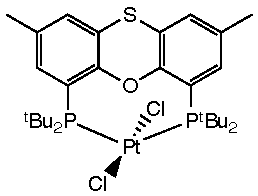
\includegraphics{../Structures/StBuPtCl2.pdf}
\end{center}
\end{structure}

\tBuThixantphos (0.198 g, 0.38 mmol) and \ce{[Pt(hex)Cl2]} (0.133 g, 0.38 mmol) were dissolved in toluene (10 mL) and heated to 50 \degC for three days, resulting in an orange solution.  The solvent was removed \emph{in vacuo} and the resulting solid was dissolved in a minimum of dichloromethane.  Diethyl ether was a small amount of oily residue became evident.  The sample was cooled to -14 \degC, resulting the title compound as red crystals (0.117 g, \fixme{\%}).

\Phosphorusintro{C6D6}
\NMRPPt{32.9}{2700}
\Protonintro{500}{C6D6}
\NMRsinglet{7.11}{\StBucH},
\NMRsinglet{6.98}{\StBuaH},
\NMRsinglet{1.86}{\StBugH},
\NMRPH{1.71}{vt}{7.3}{PCC\emph{H}\sub{3}},
\NMRbsinglet{1.56}{PCC\emph{H}\sub{3}},
\Carbonintro{125}{C6D6}
\NMRPC{155.8}{vt}{\fixme{?}}{\emph{C}O},
\NMRsinglet{134.3}{PC(Ar)\emph{C}H},
\NMRPC{131.0}{vt}{3.4}{\emph{C}(Ar)\ce{CH3}},
\NMRsinglet{129.9}{SC\emph{C}C(\ce{CH3})},
\NMRPC{124.0}{P\emph{C}(Ar)},
\NMRPC{124.5}{vt}{\fixme{?}}{\emph{C}S},
\NMRsinglet{20.3}{C(Ar)\emph{C}\ce{H3}},
\NMRPC{39.7}{vt}{\fixme{?}}{PC\emph{C}\ce{H3}},
\NMRPC{38.8}{vt}{11.1}{PC\emph{C}\ce{H3}},
\NMRPC{32.8}{vt}{3.9}{P\emph{C}\ce{CH3}},
\NMRbsinglet{30.2}{P\emph{C}\ce{CH3}},
HRMS calcd for \ce{C30H46OP2SClPt} [M-Cl]$^+$ \emph{m/z} = 745.2060; found = 745.2052.
\fixme{IR, EA, MS}

\fixme{Assigned the protonated and quaternary carbons of the tBu incorrectly}

%%%%%%%%%
%PtStBuCl PF6%
%%%%%%%%%
\subsection*{\emph{trans}-(\emph{t}-Bu-Thixantphos)platinumchloride hexafluorophosphate}
\begin{structure}[h]
\begin{center}
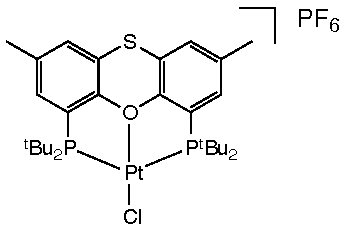
\includegraphics{../Structures/StBuPtClPF6.pdf}
\end{center}
\end{structure}

Dissolved (\tBu-Thixantphos)platinum dichloride (0.035 g, 0.045 mmol) in dichloromethane (2 mL) and added ammonium hexafluorophosphate (0.015 g, 0.090 mmol).  After 1 hour of stirring the red solution had become yellow with a white precipitate.  The solution was filtered through a plug of alumina and the solvent removed \emph{in vacuo} yielding the title compound as a yellow solid (0.030g, \fixme{\%}).  

\Phosphorusintro{CD2Cl2}
\NMRPsinglet{46.4}
\NMRPF{-144.5}{septet}{710.5}{\emph{P}\ce{F6}}
\Protonintro{500}{CD2Cl2}
\NMRsinglet{7.41}{\StBucH},
\NMRsinglet{7.11}{\StBuaH},
\NMRsinglet{2.38}{\StBugH},
\NMRPH{1.55}{vt}{8.0}{\StBuiH},
\Carbonintro{125}{C6D6}
\NMRmultiplet{157.4}{\StBueC},
\NMRsinglet{138.9}{\StBubC},
\NMRsinglet{134.4}{\StBucC},
\NMRsinglet{132.6}{\StBuaC},
\NMRmultiplet{119.8}{\StBudC},
\NMRmultiplet{119.1}{\StBufC},
\NMRPC{40.0}{vt}{10.4}{\StBuhC},
\NMRsinglet{30.1}{\StBuiC},
\NMRsinglet{20.4}{\StBugC},
\Fluorineintro{CD2Cl2}
\NMRPF{-73.4}{d}{710.6}{P\emph{F}\sub{6}}
\fixme{IR, EA, MS}

%%%%%%%%%
% PtStBuMe Cl %
%%%%%%%%%
\subsection*{\emph{trans}-(\emph{t}-Bu-Thixantphos)platinummethyl chloride}
\begin{structure}[h]
\begin{center}
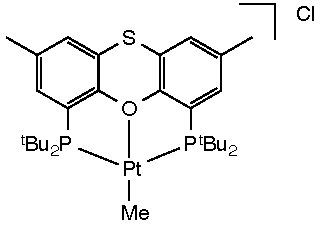
\includegraphics{../Structures/StBuPtMe.pdf}
\end{center}
\end{structure}

\Phosphorusintro{d6-acetone}
\NMRPPt{50.5}{2793.3}
\Protonintro{600}{d6-acetone}
\NMRPH{7.69}{d}{1.8}{\StBucH},
\NMRPH{7.34}{d}{1.2}{\StBuaH},
\NMRsinglet{2.42}{\StBugH},
\NMRPH{1.56}{vt}{15.6}{\StBuiH},
\NMRPH{1.94}{t}{5.5, \twoJPtH{}~=~97.4}{Pt-C\emph{H}\sub{3}},
\Carbonintro{150}{d6-acetone}
\NMRPC{153.8}{vt}{10.3}{\StBueC},
\NMRPC{137.1}{vt}{6.3}{\StBubC},
\NMRsinglet{134.4}{\StBucC},
\NMRsinglet{131.4}{\StBuaC},
\NMRPC{120.8}{vt}{31.8}{\StBudC},
\NMRPC{118.2}{vt}{7.2}{\StBufC},
\NMRPC{38.8}{vt}{20.6}{\StBuhC},
\NMRobscuredC{29.6}{\fixme{HSQC?}}{\StBuiC},
\NMRsinglet{19.2}{\StBugC},
\NMRPC{-23.8}{t}{5.6, \oneJPtC{}~=~777.2}{Pt-\emph{C}\ce{H3}}
\fixme{IR, EA, MS}

%%%%%%%%%
% PtCtBuMe Cl %
%%%%%%%%%

\subsection*{(\tBuXantphosk)-platinummethyl chloride}
\begin{structure}[h]
\begin{center}
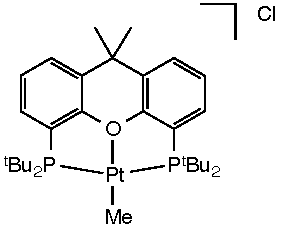
\includegraphics{../Structures/CtBuPtMe.pdf}
\end{center}
\end{structure}

\Phosphorusintro{d6-acetone}
\NMRPPt{51.0}{2788.2}
\Protonintro{500}{d6-acetone}
\NMRcoupled{8.15}{dt}{7.5, 3.7}{\CtBucH},
\NMRcoupled{8.07}{d}{7.8}{\CtBuaH},
\NMRcoupled{7.63}{t}{7.9}{\CtBubH},
\NMRPH{1.92}{t}{5.4, \twoJPtH{}~=~97.4}{Pt-C\emph{H}\sub{3}},
\NMRsinglet{1.78}{\CtBuhH}
\NMRPH{1.55}{vt}{15.4}{\CtBujH}
\Carbonintro{125}{d6-acetone}
\NMRPC{156.1}{vt}{10.2}{\CtBueC},
\NMRsinglet{135.9}{\CtBucC},
\NMRsinglet{133.2}{\CtBuaC},
\NMRsinglet{132.7}{\CtBufC},
\NMRPC{127.4}{vt}{6.6}{\CtBubC},
\NMRPC{119.7}{vt}{34.1}{\CtBudC},
\NMRPC{39.5}{vt}{21.4, \twoJPtC{}~=~43.3}{\CtBuiC},
\NMRsinglet{35.0}{\CtBugC},
\NMRsinglet{33.7}{\CtBuhC},
\NMRPC{30.4}{vt}{6.1}{\CtBujC}.
\NMRPC{-23.9}{t}{5.6, \oneJPtC{}~=~774.6}{Pt-\emph{C}\ce{H3}}

%%%%%%%%%
% PtSitBuMe Cl %
%%%%%%%%%

\subsection*{(\tBuSixantphosk)-platinummethyl chloride}
\begin{structure}[h]
\begin{center}
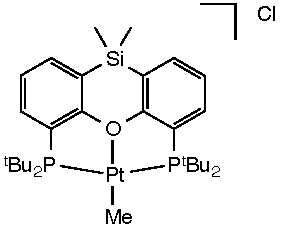
\includegraphics{../Structures/SitBuPtMe.pdf}
\end{center}
\end{structure}

%Experiment 6006
\Phosphorusintro{d6-acetone}
\NMRPPt{48.7}{2762.9}
\Protonintro{500}{d6-acetone}
\NMRmultiplet{8.39-8.36}{\SitBucH},
\NMRdd{8.11}{7.1}{1.7}{\SitBuaH},
\NMRcoupled{7.65}{t}{7.4}{\SitBubH},
\NMRcoupled{2.01}{t}{5.5 \twoJPtH{}~=~98.6}{Pt-C\emph{H}\sub{3}},
\NMRcoupled{1.55}{vt}{15.2}{\SitBuiH},
\NMRsinglet{0.59}{\SitBugH}.
\Carbonintro{125}{d6-acetone}
\NMRPC{167.3}{vt}{8.2}{\SitBueC},
\NMRPC{140.72}{vt}{\fixme{???}}{\SitBucC},
\NMRsinglet{140.67}{\SitBuaC},
\NMRPC{126.1}{vt}{6.1}{\SitBubC},
\NMRPC{123.5}{vt}{\fixme{???}}{\SitBufC},
\NMRPC{121.2}{\fixme{???}}{\fixme{???}}{\SitBudC},
\NMRPC{39.7}{vt}{21.8}{\SitBuhC},
\NMRPC{30.6}{vt}{5.6}{\SitBuiC},
\NMRsinglet{-0.5}{\SitBugC},
\NMRPC{-22.7}{t}{5.6, \oneJPtC{}~=~780.5}{Pt-\emph{C}\ce{H3}}.
HRMS calcd for \ce{C31H51OP2PtSit} [M-Cl]$^+$ \emph{m/z} = 724.2829; found = 724.2760.


\section{Palladium Complexes}
\label{section:experimental:palladium}


%%%%%%%%
% PdStBuO2 %
%%%%%%%%
\subsection*{\emph{trans}-(\emph{t}-Bu-Thixantphos)palladiumdioxygen}
\begin{structure}[h]
\begin{center}
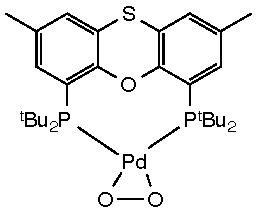
\includegraphics{../Structures/StBuPdO2.pdf}
\end{center}
\end{structure}

\fixme{check the frequency of the 500 for carbons}

\Phosphorusintro{C6D6}
\NMRPsinglet{42.9}
\Protonintro{500}{C6D6}
\NMRsinglet{7.35}{\StBucH},
\NMRsinglet{6.83}{\StBuaH},
\NMRsinglet{1.95}{\StBugH},
\NMRPH{1.46}{vt}{13.7}{\StBuiH},
\Carbonintro{125}{C6D6}
\NMRPC{155.9}{vt}{14.0}{\StBueC},
\NMRsinglet{133.6}{\StBucC},
\NMRsinglet{131.9}{\StBubC},
\NMRsinglet{128.8}{\StBuaC}
\NMRPC{127.8}{vt}{8.2}{\StBudC},
\NMRPC{124.6}{vt}{5.3}{\StBufC},
\NMRPC{35.7}{vt}{3.8}{\StBuhC},
\NMRsinglet{31.9}{\StBuiC},
\NMRsinglet{20.4}{\StBugC}
\fixme{IR, EA, MS}

%%%%%%%%
% PdStBuCl2 %
%%%%%%%%
\subsection*{\emph{trans}-(\emph{t}-Bu-Thixantphos)palladiumdichloride}
\begin{structure}[h]
\begin{center}
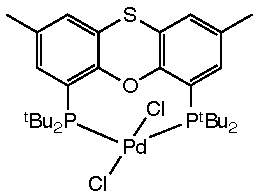
\includegraphics{../Structures/StBuPdCl2.pdf}
\end{center}
\end{structure}

\tBuThixantphos{} (0.197 g, 0.38 mmol) and \ce{[Pd(COD)Cl2]} (0.108 g, 0.38 mmol) were dissolved in toluene then heated to 40\degC for three days.  The solvent was removed \emph{in vacuo} yielding the title compound as an orange solid (0.265 g, 100\%).

\fixme{Check solvent}

\Phosphorusintro{C6D6}
\NMRPsinglet{41.9}
\Protonintro{500}{C6D6}
\NMRsinglet{7.17}{\StBucH},
\NMRsinglet{7.15}{\StBuaH},
\NMRsinglet{2.33}{\StBugH},
\NMRPH{1.59}{vt}{7.1}{\StBuiH}.
\Carbonintro{125}{C6D6}
\NMRPC{155.1}{vt}{4.8}{\StBueC},
\NMRsinglet{134.4}{\StBucC},
\NMRPC{133.4}{vt}{\StBubC},
\NMRsinglet{130.4}{\StBuaC},
\NMRPC{123.5}{vt}{12.5}{\StBudC},
\NMRsinglet{123.1}{\StBufC},
\NMRPC{39.5}{vt}{5.8}{\StBuhC},
\NMRsinglet{31.2}{\StBuiC},
\NMRsinglet{20.7}{\StBugC}.
HRMS calcd for \ce{C30H46OP2SPdCl} [M-Cl]$^+$ \emph{m/z} = 657.1468; found = 657.1446.
\fixme{IR, EA, MS}
\fixme{Check this mass spec - reprocess as Ian didn't get a good match for it}

%%%%%%%%
%PdCl2 SitBu %
%%%%%%%%
%\newpage{}
%2021
\subsection*{\emph{t}-Bu-Siixantphospalladiumdichloride} \fixme{check name}
\begin{structure}[h]
\begin{center}
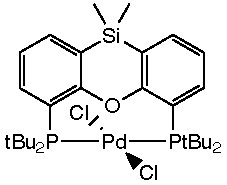
\includegraphics{../Structures/PdCl2(Si(tBu)2)_complex.pdf}
\end{center}
\end{structure}

Combined \fixme{StBu ligand} (12 mg, 0.023 mmol) and \ce{[Pd(COD)Cl2]} (7 mg, 0.025 mmol) in an \fixme{Youngs tube} and stirred at room temperature for 24 hours then 35\degC for a further 30 hours.  The solvent was removed in vacuo yielding a the title compound as a red solid \fixme{yield}.

\fixme{Include a structure}
\Phosphorusintro{CDCl3}
\NMRPsinglet{\fixme{get this value?}}
\Protonintro{500}{CDCl3}
\NMRmultiplet{7.71}{\SitBucH},
\NMRHH{7.68}{d}{7.1}{\SitBuaH},
\NMRHH{7.33}{t}{7.3}{\SitBubH},
\NMRPH{1.60}{vt}{7.3}{\SitBuiH},
\NMRsinglet{0.52}{\SitBugH}.
\Carbonintro{125}{CDCl3}
\NMRPC{165.1}{vt}{\fixme{?}}{\SitBueC},
\NMRsinglet{137.6}{\SitBucC},
\NMRsinglet{136.9}{\SitBuaC},
\NMRsinglet{124.9}{\SitBufC},
\NMRsinglet{123.1}{\SitBubC},
\NMRPC{121.8}{vt}{13.4}{\SitBudC},
\NMRPC{39.6}{vt}{6.3}{\SitBuhC},
\NMRPC{31.1}{vt}{2.7}{\SitBuiC},
\NMRsinglet{-2.0}{\SitBugC}.
\fixme{IR, mass spec, EA}
\fixme{Check the solvent}

%%%%%%%%%
% PdStBuClPF6%
%%%%%%%%%
\subsection*{\emph{trans}-(\emph{t}-Bu-Thixantphos)palladiumchloride hexafluorophosphate}
\begin{structure}[h]
\begin{center}
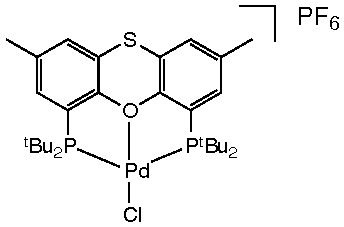
\includegraphics{../Structures/StBuPdClPF6.pdf}
\end{center}
\end{structure}

\fixme{Check solvent}

\Phosphorusintro{CD2Cl2}
\NMRPsinglet{56.4}
\NMRPF{-144.5}{septet}{710.5}{\emph{P}\ce{F6}}
\Protonintro{500}{CD2Cl2}
\NMRPH{7.36}{d}{2.0}{\StBucH},
\NMRsinglet{7.15}{\StBuaH},
\NMRsinglet{2.38}{\StBugH},
\NMRPH{1.58}{vt}{8.2}{\StBuiH},
\Carbonintro{125}{C6D6}
\NMRPC{154.86}{vt}{6.5}{\StBueC},
\NMRPC{138.3}{vt}{\fixme{?}}{\StBubC},
\NMRsinglet{134.6}{\StBucC},
\NMRsinglet{132.6}{\StBuaC},
\NMRsinglet{119.1}{\StBufC},
\NMRPC{118.7}{vt}{10.8}{\StBudC},
\NMRPC{40.2}{vt}{7.2}{\StBuhC},
\NMRsinglet{30.1}{\StBuiC},
\NMRsinglet{20.4}{\StBugC}
\Fluorineintro{CD2Cl2}
\NMRPF{-73.4}{d}{710.6}{P\emph{F}\sub{6}}
\fixme{IR, EA, MS}

%%%%%%%%%
% PdStBuOAc2 %
%%%%%%%%%
\subsection*{\emph{trans}-(\emph{t}-Bu-Thixantphos)palladiumdiacetate}

\begin{structure}[h]
\begin{center}
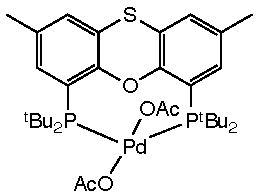
\includegraphics{../Structures/StBuPdOAc2.pdf}
\end{center}
\end{structure}

\Phosphorusintro{C6D6}
\NMRPsinglet{33.7}
\Protonintro{500}{C6D6}
\NMRPH{7.07}{d}{2.0}{\StBucH},
\NMRsinglet{6.83}{\StBuaH},
\NMRsinglet{1.89}{\StBugH},
\NMRbsinglet{1.42}{\StBuiH},
\fixme{Peak for acetates?}
\Carbonintro{125}{C6D6}
\NMRbsinglet{177.7}{O\emph{C}(O)\ce{CH3}}
\NMRPC{156.3}{vt}{8.4}{\StBueC},
\NMRPC{134.4}{d}{13.9}{\StBucC},
\NMRsinglet{132.9}{\StBubC},
\NMRsinglet{129.9}{\StBuaC},
\NMRPC{123.5}{vt}{\StBufC},
\NMRPC{120.3}{vt}{22.4}{\StBudC},
\NMRPC{37.0}{vt}{10.2}{\StBuhC},
\NMRbsinglet{30.3}{\StBuiC},
\NMRbsinglet{24.3}{OC(O)\emph{C}\ce{H3}}
\NMRsinglet{20.3}{\StBugC}
\fixme{IR, EA, MS}

\section{Rhodium complexes}

%%%%%%%%
%Rh(CtBu)Cl %
%%%%%%%%

\subsection*{(\tBuXantphosk-\emph{P,O,P})-rhodiumchloride}

\begin{structure}[h]
\begin{center}
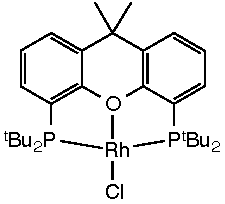
\includegraphics{../Structures/RhCl(CtBu).pdf}
\end{center}
\end{structure}

\Phosphorusintro{C6D6}
\NMRRhP{47.7}{142.3}
\Protonintro{500}{C6D6}
\NMRcoupled{7.78}{d}{7.3}{\CtBucH},
\NMRcoupled{7.01}{d}{7.6}{\CtBuaH},
\NMRcoupled{6.80}{t}{7.7}{\CtBubH},
\NMRPH{1.68}{vt}{13.4}{\CtBujH},
\NMRsinglet{1.16}{\CtBuhH}.
\Carbonintro{500}{C6D6}
\NMRPC{158.9}{vt}{16.3}{\CtBueC},
\NMRsinglet{133.6}{\CtBucC},
\NMRsinglet{131.6}{\CtBufC},
\NMRsinglet{127.7}{\CtBuaC},
\NMRPC{125.7}{vt}{12.0}{\CtBudC},
\NMRsinglet{123.8}{\CtBubC},
\NMRPC{37.6}{vt}{10.1}{\CtBuiC},
\NMRsinglet{32.5}{\CtBugC},
\NMRsinglet{33.8}{\CtBuhC},
\NMRPC{30.8}{vt}{7.7}{\CtBujC}.

\newpage{}
\section{Things that need to be fixed or added for final thesis}
\begin{itemize}
\item{Check that negative sign is actually negative and not a hyphen or other type of dash}
\item{Check freezer temperature for recrystallisations, approx -14\degC}
\item{Include reaction between Pt(tBu-thixantphos)O2 and PTA}
\item{Include reaction between Pt(COD)2 and tBu-thixantphos}
\item{Make sure all captions have full stops}
\item{Check that bis and cis etc. are all italics or not as necessary, bis should not be, cis and trans should be.  Also sec should be \emph{sec} not s as s is stereochemical}
\item{Double bonds look better in ce rather than as equals}
\item{Check that the correct measurements for virtual triplets are made}
\item{Correct my nmr stuff such that a is actually labelled correctly}
\item{Note that tBu-xantphos is also used for the tBu on the backbone...}
\item{Should it be square-planar or square planar?}
\item{A note on nomenclature tBu-xantphos means two different things and tBu-xantphos vs Ph-xantphos}
\item{Consider using mg for NMR scale reactions}
\item{Check that the silver complexes have complete coupling data, as much as possible}
\item{Check if X-ray should be capitalised, it should so make sure that it is}
\end{itemize}

\newpage{}
\section{Lab work that still needs to be done}
\begin{itemize}
\item{Get 31P chemical shift for PdO2 complex in acetone - sample 4042}
\item{React dioxygen complex with CO2 to get a peroxycarbonate c.f. Goel1983b}
\item{See if reaction of the dioxygen complex with hydrogen results in the reduction to platinum(0), c.f. Sergeev2010}
\begin{itemize}
	\item{Has been reacted at 1 atm and RT, with no reaction observed}
	\item{Repeat at higher pressure}
\end{itemize}
\item{Repeat reaction of dioxygen complex with CO}
	\begin{itemize}
	\item{Get 13C shift of the metallated carbon - seems very likely to be 15.5 ppm}
	\item{Run long HSQC to low ppm to see if I can identify the protons - unsuccessful}
	\item{Run VERY long 13C to try and see platinum satellites - very unlikely - should be able to see them, but no luck}
	\item{React metallated product with methane and hydrogen}
	\end{itemize}
\item{Purifiy the StBu selenide then get and assign full set}
\item{Repeat reaction with Pt(C2H4)3 and StBu to in sealed tube to prevent oxidation and check that everything that is made is the ethene complex}
\item{Repeat reaction with Pt(COD)2 and StBu in a sealed NMR tube to ensure that no COD complex forms}
\item{Repeat reaction with Rh(COE)2Cl and StBu in acetone and see if the Rh(III) complex forms faster - check the NMR of 4037 to see any sign of complexed acetone}
%\item{Complete reaction between Ir(COE)2Cl and StBu}
\item{React CtBu and SitBu with Pt(nb)3 as comparisons or sterics etc.}
\item{React PtMeStBu complex with PF6 to confirm the structure as without a chloride}
\item{Calculate structure of Pt(POP)Me complex to see if an agostic is present}
\item{React C bridged ligand with Pt(nb)3}
\item{Investigation of PP distance in the ligands, is the Si ligand to hard to make because of a lithium complex with the phosphines, according to David's thesis page 47 the smaller the distance the greater the bond strength}
%\item{React ligand with RhCl3 to see if the degradation product is a RhCl3 complex}
\end{itemize}

\section{Lab work that would be nice to do}
\begin{itemize}
\item{VT NMR on all three protonated ligands}
	\begin{itemize}
	\item{Get coalescence temperatures as an indication of the amount of exchange that is occurring}
	\end{itemize}
\item{VT NMR with the lithiated ligand to try and get P-Li coupling constant}
\item{React 14-electron complex with silane and HCl to try and identify the unknown hydride that forms when reacting with Pt(COD)2 or Pt(nb)3}
\item{Palladium analogue of PtMe}
\item{Protonation of PtMe complex}
\end{itemize}

\newpage{}
\section{Home work that still needs to be done}
\begin{itemize}
\item{Get mercury working on laptop}
	\begin{itemize}
	\item{Find out how to measure backbone bending}
	\end{itemize}
\end{itemize}

\section{Desk work that still needs to be done}
\begin{itemize}
\item{Complete bite-angle calculations}
\item{Check for the VT that I did on the protonated ligand}
\item{Look up structures for Pt(P)2 on scifinder and CCD}
	\begin{itemize}
	\item{Check if there are any with diphosphines, van Leeuwens review suggested that there were not}
	\end{itemize}
\item{Check 600 MHz for a carbon on 4019 after 18/4}
\item{Check solubility of CO across different temperatures}
\item{Look at 4027 (oxidation of StBu) to try and find evidence of S oxidation}
\item{Look at VT on 4029 - dichloride complex}
\item{Fully assign 4031 (CtBu selnide?)}
\item{Assign IR stretches}
	\begin{itemize}
	\item{It may be necessary to compare with calculated IRs}
	\end{itemize}
\item{Check the integrals for nb, ethene and COD complexes to go into thesis}
\item{ORTEP diagrams of crystal structures}
\item{Update the synthesis books}
\item{Read up on iridium hydride metallation stuff, see Kranenburg1995 for an unusual Rh complex}
\item{Read Mora2008 to get ideas for catalysis}
\item{Read up on through space NMR coupling with relation to the protonated ligands - ask Robin?}
\item{Get mestranova NMR stuff for the VT on the dichloride (4009?) that I did}
\end{itemize}

%\subsection*{2,4-Di(carbomethoxy)-1,5-bis(\emph{p}-dimethylaminophenyl)-penta-1,4-dien-3-one}

%\begin{structure}
%\begin{center}
%\includegraphics[scale=1.2]{structures/dba436}
%\end{center}
%\end{structure}


%\noindent Dimethyl 1,3-acetonedicarboxylate (3.5~g, 0.02 mol), \textit{p}-di\-methy\-lamino\-benz\-aldehyde (6.0~g, 0.04 mol), piperidine (0.45~\cm, 4.6~mmol) and glacial acetic acid (0.30~\cm, 5.2~mmol) were combined in benzene (60~\cm) in a 250~\cm{} round bottom flask in the air.  The flask was equipped with a Dean-Stark trap to measure the volume of water being eliminated during the course of the reaction.  The trap was in turn equipped with a condenser, and the reaction mixture was heated under reflux for 1 day.  About 0.7~\cm{} of water were collected in the Dean-Stark trap indicating that the reaction was complete.  The solvent was removed \textit{in vacuo} to yield a dark red oil.  The oil was washed with petroleum ether several times then taken up in benzene.  The mixture was stirred at room temperature for several hours during which yellow crystalline solid precipitated out as the oil slowly dissolved.  The solid was filtered, washed with benzene and dried in the air
%(7.5~g, 86\%); 
%mp 124.5-124.8\degC{} (from benzene);
%(Found: C, 69.2; H, 6.5; N, 6.4. \ce{C25H28N2O5} requires C, 68.8; H, 6.5; N, 6.4\%);
%\numax(KBr)/\percm{} 1732, 1719, 1701, 1693, 1572, 1526, 1373, 1189 and 1158;  
%\dH(300~MHz; \ce{C6D6}; \ce{Me4Si}) 
%2.18 (6 H, s, \ce{NMe2}), 
%2.19 (6 H, s, \ce{NMe2}), 
%3.43 (3 H, s, OMe), 
%3.69 (3 H, s, OMe), 
%6.12 (2 H, d, \JHH{} 9.0, \textit{m}-H), 
%6.23 (2 H, d, \JHH{} 9.0, \textit{m}-H), 
%7.31 (2 H, d, \JHH{} 9.0, \textit{o}-H), 
%7.62 (2 H, d, \JHH{} 9.0, \textit{o}-H), 
%7.88 (1 H, s, CH=CH) and 
%8.32 (1 H, s, CH=CH);  
%\dC(75~MHz; \ce{C6D6}; \ce{Me4Si}) 
%39.15 (2 C, s, \ce{NMe2}), 
%39.17 (2 C, s, \ce{NMe2}), 
%51.8 (1 C, s, OMe), 
%52.0 (1 C, s, OMe), 
%111.8 (1 C, s, \textit{m}-\ce{C6H4}), 
%112.1 (1 C, s, \textit{m}-\ce{C6H4}), 
%120.9 (2 C, s, \ce{C6H4}), 
%121.2 (2 C, s, \ce{C6H4}), 
%132.5 (2 C, s, \textit{o}-\ce{C6H4}), 
%133.2 (2 C, s, \textit{o}-\ce{C6H4}), 
%143.7 (1 C, s, \textit{p}-\ce{C6H4}), 
%143.9 (1 C, s, \textit{p}-\ce{C6H4}), 
%166.5 (1 C, s, COO), 
%169.3 (1 C, s, COO) and 
%193.8 (1 C, s, CO);
%\textit{m/z} (ESI) 459.1000 (\MplusNa. \ce{C25H28N2O5Na} requires 459.1896).